\documentclass[12pt,preprint]{aastex}
\usepackage{float,amsmath}
%\usepackage[margin=1in]{geometry}
%\usepackage{titlesec} %used to format titles
\usepackage{graphicx} %for handling figures
%\usepackage[none]{hyphenat} %disallows hyphenated words
\newcommand{\vdag}{(v)^\dagger}
\newcommand{\volt}{{v}}
\newcommand{\vis}{{V}}
\newcommand{\sky}{{\rm sky}}
\newcommand{\bmvolt}{{a}}
\newcommand{\bm}{{A}}
\newcommand{\thhat}{{\hat\theta}}
\newcommand{\fngexp}{{e^{\frac{2\pi i\nu\vec{b}\cdot\thhat}{c}}}}
\newcommand{\ifngexp}{{e^{-\frac{2\pi i\nu\vec{b}\cdot\thhat}{c}}}}
\newcommand{\myemail}{skywalker@galaxy.far.far.away}

%\usepackage{cite}

%\citestyle{aa}
\shorttitle{HERA dish reflectometry }
\shortauthors{Patra et al.}

\begin{document}

\title{Effect of multiple reflection of the sky signal off the HERA element on the measurements of 21cm power spectrum} 
%\maketitle

\author{Nipanjana Patra\altaffilmark{1} }
\email{Contact author email: nipanjana@berkeley.edu}


\author{Zaki Ali\altaffilmark{1}, Carina Cheng\altaffilmark{1}, Dave DeBoer\altaffilmark{1}}
\author{Gilbert Hsyu\altaffilmark{2}, Tsz Kuk Leung\altaffilmark{2}, Aaron Parsons\altaffilmark{1}}
% XXX add all members of HERA collaboration
% XXX suggest Patra, Parsons, Ali, DeBoer, Cheng, Leung, Hsyu, alphabetical

\altaffiltext{1}{University of California, Berkeley, nipanjana@berkeley.edu}
\altaffiltext{2}{To be inserted}

\begin{abstract}
\end{abstract}


\section{Introduction}

Since it was first proposed in \citet{shaver_et_al1999}, measuring 21~cm
emission from neutral hydrogen in our early universe has gained attention as a
powerful probe of both cosmology and astrophysics.  While the science case for
21~cm cosmology, particularly during the Epoch of Reionization, is well
established (see, e.g.,
\citealt{furlanetto_et_al2006,morales_wyithe2010,furlanetto_loeb2014,pritchard_loeb2014}),
the technical path toward measuring this signal has been more problematic.  The
weakness of this hyperfine line keeps the 21~cm signal below opacity throughout
cosmological history, but it also creates sensitivity and calibration
challenges that have yet to be fully solved.  With noise temperatures dominated
by sky noise \citep{XXX} and foregrounds four to five orders of magnitude
brighter than the signal \citep{XXX}, 
sky-averaged 21~cm monopole experiments such as
(EDGES; \citealt{XXX}),
(BIGHORNS; \citealt{XXX}),
(SARAS; \citealt{patra_et_al2014}),
(SCIHI; \citealt{voytek_et_al2014}),
(HyPerion; \citealt{presley_et_al2015})
% XXX others?
and 21~cm reionization power spectrum experiments such as
the LOw Frequency ARray (LOFAR; \citealt{XXX}),
the Murchison Widefield Array (MWA; \citealt{XXX}),
the Giant Metre-wave Radio Telescop (GMRT; \citealt{XXX}),
the Donald C. Backer Precision Array to Probe the Epoch of Reionization (PAPER; \citealt{parsons_et_al2010}),
the Hydrogen Epoch of Reionization Array (HERA; \citealt{XXX}),
and the future Square Kilometre Array (SKA; \citealt{XXX})
must
furnish both collecting area and foreground suppression at levels significantly
beyond anything previously achieved in radio telescopes operating below 1 GHz.

One of the most problematic effects facing these experiments is instrument
chromaticity.  The spectral dimension of 21~cm reionization experiments is of vital
importance; for line emission, this coordinate translates to a line-of-sight distance
that can be used to construct three-dimensional maps (and power spectra) of emission,
as well as probe the evolution of 21~cm emission over cosmological timescales.
The evolving response of a radio telescope --- either a single dish
or an interferometer --- versus spectral frequency modulates spectrally smooth foregrounds,
contaminating spectral modes that might
otherwise be used to measure reionization \citep{XXX}.  Moreover, the chromaticity of
a telescope's response scales linearly with diameter, putting the
needs of foreground suppression and signal sensitivity in direct tension with one
another.

A major step forward for the field of 21~cm cosmology has been the development
of a mathematical description of telescope chromaticity, how it varies with
element separation (or telescope diameter), and what it implies for distinguishing
foreground emission from the cosmological 21~cm signal \citep{XXX}.  The ``wedge'', as it is
colloquially known, describes a linear relationship between the separation between elements
in an interferometric baseline and the maximum line-of-sight Fourier mode\footnote{Assuming
a flat sky, and using appropriate
cosmological scalars,
the spectral axis, $\nu$, and angle on the sky, $\vec\theta$, translate to coordinates in
a three-dimensional volume at cosmological distances.  In describing the spatial power spectrum of
emission in this volume $P(\vec k)$, we use the three-dimensional wave vector 
$\vec k\equiv(k_\parallel,\vec k_\perp)$, where $k_\parallel$ is aligned with the
spectral axis $\nu$, and $\vec k_\perp$ lies in the plane of the sky.}
that may be occupied by smooth spectrum foreground emission.  At low-order $k_\parallel$ modes
within the limits of the wedge,
foreground contamination may be suppressed through a combination of calibration and model 
subtraction.  However, calibration or modeling errors rapidly re-establish the characteristic
wedge pattern.  Outside of the wedge, foreground contamination drops rapidly 
\citep{pober_et_al2013,thargarajan_et_al2015}, provided that the spectral responses
of antenna elements and analog electronics are sufficiently smooth\footnote{Here, we distinguish
the chromaticity of the elements in isolation from the chromaticity inherent to
element separation in an interferometric baseline.}.  In promising avoidance-based
foreground strategy employed by PAPER \citep{parsons_et_al2014,ali_et_al2015}, these modes
may be targeted as the lowest risk path for contraining 21~cm reionization in the near term.

In this paper, we examine the performance of a new prototype HERA element in the context of
this new wedge-based framework.  In coordination with \citet{XXXsisterpapers}, we compare 
reflectometry measurements with
a specification for the spectral performance of an element, given models of the relative brightness of
foreground and 21~cm reionization modes in $k$-space.  
% XXX document map



The efficacy of the techniques of foreground removal from the measured data critically limits the 21~cm power spectrum measurements. The delay transformation technique of foreground removal, introduced by  \citep{ParsonsBacker2009,Parsons2012} computes the Fourier transform of the visibility measured by an interferometer and produces a spectrum, referred to as delay spectrum hereafter, which is a function of the geometric time delay corresponding to the physical length of the baseline between two antennas. For the visibilities measured over a wide field across wide frequency bandwidth, the delay spectrum is constituted by the instrument response, the foreground signal and 21cm power spectrum, hereafter referred to as EoR signal.
%The complex visibility measured by an interferometer is a convolution of the instrument response with the true sky response in the UV plane. Therefore, when Fourier transformed, the delay spectrum is the multiplication of the sky response with the instrument response in the delay domain.
The technique exploits the smooth spectral characteristics of the foreground and for a widefield wide bandwidth visibility measurement by an interferometer with a baseline $b$, confines the foreground contribution to the computed delay spectrum within the largest possible time delay $\tau = b/c$ corresponding to the given baseline length. Such techniques also assumes a spectrally smooth instrumental response whose contribution to the measured data, much as the contribution of the smooth spectrum foreground, also has an upper bound in the delay space imposed by the largest geometric delay of the given baseline. 
Beyond this limit, for an ideal system performance, the delay spectrum would be dominated by any wideband signal across the sky with spectral and spatial fluctuation over small scale such as the EoR signal and therefore, could be detectable.\\ 
The interaction between the sky signal and instrument response can alter the relative contribution of the foreground, instrument response and the EoR signal at a given delay and thus influence the detectability of the EoR signal. Such interactions may cause the foreground and systematics to spill over at higher delays and thus push the upper limit of the foreground and systematic contaminated delay modes to much higher delays. In this process, the EoR signal over large spatial scale will be lost.

 The Hydrogen Epoch of Reionization Array (HERA) is a proposed array consisting of 568 14-m dishes in South Africa which will measure the 21~cm power spectrum between 100 to 200~MHz . In this paper, we investigate the performance of the individual HERA elements and resulting contribution of the instrument response to the delay spectrum. Reflectometry measurements  are carried out across wide bandwidth on a prototype HERA element in Green
Bank, WV (Figure \ref{fig:heradish}) and the results are interpreted in the light of delay spectrum technique. Section 2 describes the delay spectrum for the ideal and non-ideal performance of a two element interferometer. Reflectometry measurements are described in section 3. Section 4 qualifies the performance of the HERA element as an interferometer for detection of the 21~cm power spectrum.


\begin{figure}[ht!]
\centering
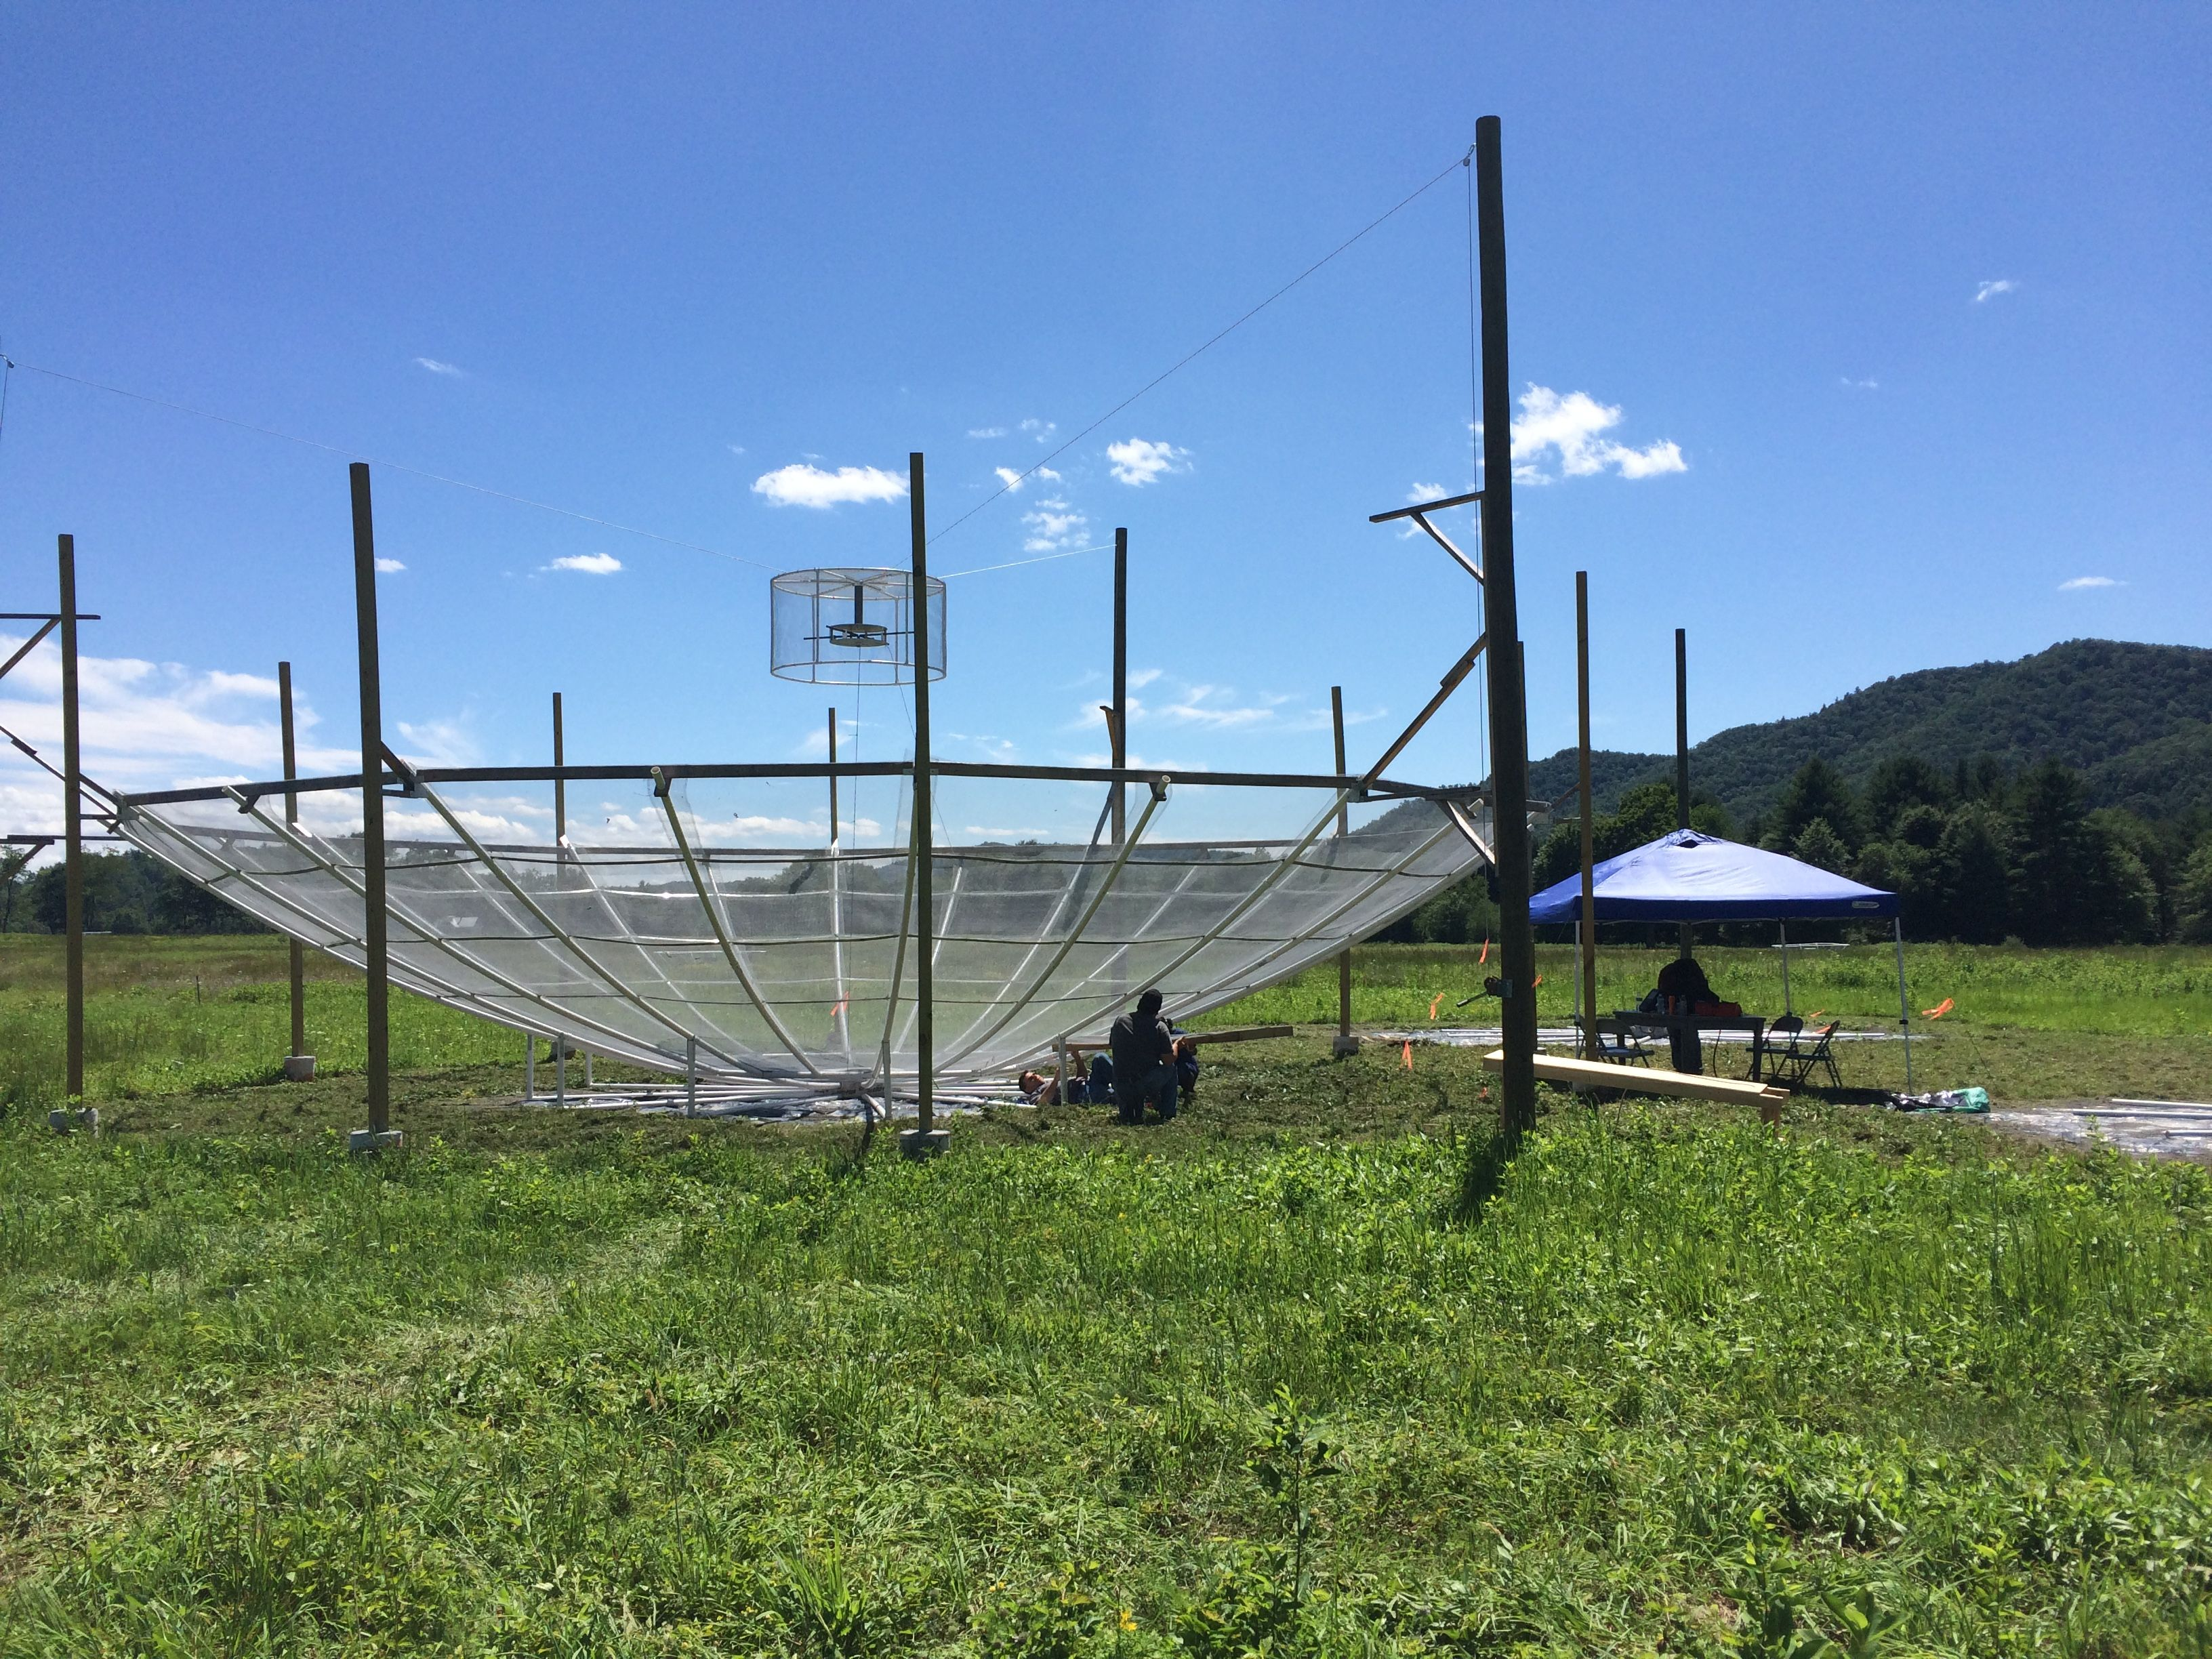
\includegraphics[trim={2cm 20cm 30cm 15cm},clip, totalheight=0.3\textheight]{plots/heradish.jpg}
\caption{HERA dish and feed at the Green Bank NRAO site.}
\label{fig:heradish}
\end{figure}

\section{Visibility measurements by a two element interferometer}

Consider a two element interferometer with a baseline $\vec b$ and antenna field pattern $A(\thhat, \nu)$. If we denote the electric field sky signal in direction $\thhat$ by $\volt_\sky(\vec \theta, \nu)$ and the receiver noise of each element as $\volt_{rec}(\nu)$ then the voltage output of each antenna may be written as,  
\begin{equation}
\volt_{1}(\thhat, \nu) = \bmvolt_{1}(\thhat,\nu)\volt_\sky(\thhat,\nu)\nonumber\\
\end{equation}
\begin{equation}
\volt_{2} (\thhat, \nu)= \bmvolt_{2}(\thhat,\nu)\volt_\sky(\thhat,\nu)\fngexp\nonumber\\
\end{equation}
where $\bmvolt_{1}(\thhat,\nu)$ and $\bmvolt_{2}(\thhat,\nu)$ are the electric field response patterns 
of the two antennas.
Hence, the time averaged visibility measured by the interferometer may be written as, 
\begin{equation}
\vis(\vec b, \nu) =  \int  \volt_{1}(\thhat,\nu)  \volt_{2}^{*} (\thhat, \nu) \ifngexp d\Omega 
\label{eq1}
\end{equation}

We define antenna cross power pattern as  $\bm(\thhat,\nu)=\bmvolt_{1}(\thhat,\nu)\bmvolt_{2}^{*}(\thhat,\nu)$ and denote the sky intensity as  $I_\sky(\thhat,\nu)=\volt_\sky(\thhat,\nu)\volt_\sky^{*}(\thhat,\nu)$. Hence, 
\begin{equation}
\vis(\vec b,\nu) = \int \bm(\thhat, \nu) I_\sky(\thhat,\nu) \ifngexp d\Omega
	%	& = & \int B(l,m, \nu) I_{sky}(l,m,\nu) exp(-2\pi i \nu \tau_{g} ) dl dm \nonumber\\
 	%	& = & B(\vec u,\nu) \ast P_{sky}(\vec u,\nu ) \nonumber\\
	%	& = & B(\nu { |\vec b| \over c} , \nu) \ast P_{sky}(\nu { |\vec b| \over c} , \nu) \nonumber\\
	%	& = & B(\tau_{g}, \nu) \ast P_{sky}(\tau_{g} , \nu)	
\label{eq2}
\end{equation}

%i.e, the complex visibility is the Fourier transform of the product of the antenna beam pattern with the sky angular power spectrum. In other words, it is the convolution of the Fourier transform of the antenna power pattern with the Fourier transform of the sky. The complex visibility measured by an interferometer with a given baseline length has explicit dependence on frequency as well as implicit frequency dependence through the spatial frequency $\vec u = \nu { \vec b \over c}$ component. Since $\vec u $ is the For a given baseline length $|\vec b|$, the visibility measured at various frequencies are not only the function of frequencies but also samples different $\vec u$ in the uv space. Delay transformation technique takes the visibility measurements at different frequencies and Fourier transforms the complex visibilities. If we defineI_{sky} the Fourier conjugate of the frequency axis as $\tau$ then the equation could be written as, 
In \citet{parsons_et_al2012a}, the Fourier transform of the visibility along the frequency axis was introduced,
resulting in the delay spctrum:
\begin{eqnarray}
\tilde V(\vec b, \tau) & = & \int\!\!\int{\bm(\thhat,\nu) I_\sky(\thhat,\nu) \ifngexp d\Omega~e^{-2\pi i\nu\tau}d\nu}\nonumber\\	                        & = &   \int \left [ A(\vec b, \tau)\ast I_{sky}(\vec b, \tau) \ast \delta( \vec b, \tau )\right ] d\Omega 
\label{eq3}
\end{eqnarray}
% XXX rethink how to express this equation (not correct about integrated over all sky)
% XXX define tau_g
where $\tau_{g} = {\vec b \cdot \thhat \over c}$. The convolution is carried out along the $\tau$ axis which is Fourier conjugate of the frequency $\nu$. In words, the sky delay spectrum is convoluted with the delay spectrum of the instrument. In the delay domain, the sky spectrum from any direction $\thhat$ would be located at $\tau = {\vec b \cdot \thhat \over c}$. Since the maximum geometric delay possible for a given base line would be    and is centred at a delay $\tau_{g}$. The projected geometric delay $\tau_{g}$ for a given baseline can vary from 0 to $\tau_{g}$. Also, due to frequency dependence of the sky signal, the delay spectrum of the sky spills over the delay $\tau> \tau_{g}$ with decaying amplitude [Ref to the figure Parsons12]. Sky delay spectrum $I_{sky}(\tau)$ is contributed by the foreground  $I_{fg}(\tau)$ and the 21~cm power spectrum $I_{21}(\tau)$. Since $I_{fg}$ is spectrally smooth, whereas $I_{21}$ contains spectral structures, for wideband measurements, the relative strength of the smooth spectrum foreground with respect to the delay spectrum of the $I_{21}$ reduces at higher delays and, therefore, at higher delays, the 21~cm delay spectrum is detectable.  \textbf{[ Reference to Nithya's foreground simulation work, reference to any plots on the relative contribution of the  foreground and EoR signal. ]}


\section{Effects of additional reflections of the sky signal between the parabolic dish and the feed on the measured visibility}
 Plane waves incident on a parabolic dish are focussed at the feed which is kept at the focal plane of the dish. The mismatch between the impedance of free space and the feed and transmission line results in a partial coupling of the sky signal into the feed while the rest is reflected off the feed. The reflected signal illuminates the dish and most of it is reflected back into the space. However, a part of it reflects back and forth several times in between the feed and the vertex of the dish which is shadowed by the feed (dashed blue arrows in Figure \ref{fig:cartoon}). Such reflections generate multiple copies of the incident sky signal of reduced strength at various time/phase and thus produces spurious correlations in the visibilities of interferometric data. In this section we compute the visibility of a two element interferometer accounting for the additional reflections of the sky signal in between the feed and the dish vertex and the corresponding effects on the delay spectrum. 

\begin{figure}[ht!]
\centering
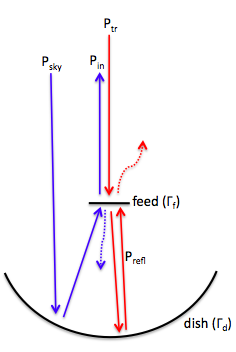
\includegraphics[totalheight=0.35\textheight]{plots/reflection_cartoon.png}
\caption{The blue solid lines represent an original sky signal entering the
feed. A small percentage of it (dashed blue) is reflected off the dish, and it
is these reflections that we are concerned about. In our measurements however,
the reflections measured contain most of the original pulse signal (solid red),
so it is crucial to adjust for this difference in our analysis.}
\label{fig:cartoon}
\end{figure}

Consider again a two element interferometer as described in section 2. Two antennas are assumed to be exactly identical so that their electrical parameters are same. We denote the voltage reflection coefficient of each feed by $\Gamma_{f}$. The voltage reflection coefficient of the reflector dish is denoted by $\Gamma_{d}$. Upon first incidence of the sky signal onto the dish, the entire sky signal would be reflected and focussed onto the feed. Hence, for first incidence $\Gamma_{d}=1$. Sky signal that would return to the dish after successive reflections off the feed and the dish is only reflected from a small area around the vertex of the dish and therefore, $\Gamma_{d}<1$. In our analysis, we consider one reflection of the sky power from the feed and subsequent reflection off the dish as one single reflection. If the focal length of the dish is $l$, assuming the feed is located at the focus, the roundtrip delay after first reflection will be $\Delta \tau = {2l \over c}$. 


\subsection{Effect of first order reflections on visibility and delay spectrum}
Upon first incidence of the sky signal $V_{sky}$, $\Gamma_{f}$ fraction of the voltage is reflected off the feed while $(1-\Gamma_{f})$ fraction is coupled to the feed. The reflected voltage then further reflected off the dish and $(1-\Gamma_{f}) $ fraction of it reenters the feed with a roundtrip time delay $\Delta \tau$. Hence, the net voltage at the output of the two antennas could be written as,    
\begin{eqnarray}
V_{1} & = & A V_{sky}(1-\Gamma_{f}) + A V_{sky} \Gamma_{f} \Gamma_{d} e^{2\pi i\nu \Delta \tau}  (1-\Gamma_{f})^{2}\nonumber\\
         & = & A V_{sky} (1-\Gamma_{f}) \left [ 1+ (1-\Gamma_{a})\Gamma_{f} \Gamma_{d} e^{2\pi i\nu \Delta \tau} \right]\nonumber\\
\label{eq4}
\end{eqnarray}
\begin{eqnarray}
V_{2} & = & A V_{sky}(1-\Gamma_{f}) + A V_{sky} \Gamma_{f} \Gamma_{d} e^{2\pi i\nu \Delta \tau} (1-\Gamma_{f})^{2}exp({2\pi i \nu \vec{b}.\hat{s} \over c} )\nonumber\\
         & = & A V_{sky} (1-\Gamma_{f}) \left [ 1+(1-\Gamma_{a}) \Gamma_{f} \Gamma_{d} e^{2\pi i\nu \Delta \tau}  \right]exp({2\pi i \nu \vec{b}.\hat{s} \over c} )\nonumber\\
\label{eq5}
\end{eqnarray}
Frequency as well as angular dependence of the quantities are not written explicitly for notational simplicity. 
The two antennas are assumed to have identical beam pattern which is $A_{1}=A_{2} =A$. We also absorb the common gain term $(1-\Gamma_{f})$ with antenna response $A$ and denote them as $A_{f}= A(1-\Gamma_{f})$ here after. Hence, the complex visibility could be, 

\begin{eqnarray}
V e^{i\phi}(\nu) & = & \int V_{1}V_{2}^{*} d\Omega \nonumber\\
		        & = & \int |A_{f}|^{2}|V_{sky}|^{2} |\left [ 1+(1-\Gamma_{f}) \Gamma_{f} \Gamma_{d} e^{2\pi i\nu \Delta \tau}  \right]|^{2} exp({2\pi i \nu \vec{b}.\hat{s} \over c} ) d\Omega
\label{eq6}		        
\end{eqnarray}


 Furthermore, combining all the terms that contain instrument response we define a common instrument parameter, written as, 
\begin{eqnarray}
\Sigma(\vec \theta, \nu) & = & |A_{f}|^{2} |\left [ 1+ (1-\Gamma_{f}) \Gamma_{f} \Gamma_{d} e^{2\pi i\nu \Delta \tau} \right]|^{2}\nonumber\\
 	    & = &  |A_{f}|^{2}  \left[ 1+ |(1-\Gamma_{f})|^{2}|\Gamma_{f}|^{2}|\Gamma_{d}|^{2} + 2 \Re \left ( (1-\Gamma_{f})\Gamma_{f}\Gamma_{d} e^{2\pi i\nu \Delta \tau} \right) \right] 
\label{eq{7}}	    
\end{eqnarray} 

Instrumental response function acquires additional terms arising due to correlation between the directed and reflected component of the sky signal. The total visibility at any frequency would be the sum of the three visibilities contributed by three sources of correlated power. First term in the square bracket represents the cross correlation between the two antenna outputs contributed by the sky signal upon first direct incidence. The second term results from the cross correlation between two reflected signals in each antenna.The last term represents the cross correlation between the first direct incident signal of one antenna and the first reflected signal from the other antenna and vice versa.

Fourier transform of this visibility spectrum along the frequency axis results in the delay spectrum. 
 Fourier transform of the visibility contributed by any two voltage components from two antennas with no mutual delay is centred at a delay $\tau = \tau_{g}$ in the delay spectrum whereas any two voltage components from two antennas components having a mutual delay of $\Delta \tau$ will be centred at $\tau_{g} +\Delta \tau$. Therefore, the correlation between the reflected signal  from the feed and subsequently from the dish with the direct signal thus extends the foreground response to delays beyond the maximum geometric delay for a given baseline and contaminates the delay mode where 21~cm delay spectrum could potentially be detected. Also, any reflections arriving at the feed at any non-zero  value of the delay $\Delta \tau$ which could be the result of reflections from the feed structures would also generate non zero delay response at those delays. 
If the dish vertex is so constructed such that the reflection from the dish vertex is negligible i.e, $\Gamma_{d}<<1\ or = 0$ then the second and the third term of the $\Sigma$ vanish. Also, if we assume a $\Gamma_{a} =-10dB$ and $\Gamma_{d}= -20dB$, the second term in the expression of $\Sigma(\vec \theta, \nu)$ becomes negligible compared to the first and the third term of the expression and, therefore, can be neglected. \\

\subsection{Effect of higher order reflection on the delay spectrum} 
Correlation between the higher order reflections of the signal in any antenna with the direct component of the other would result in a delay response at integral multiple of $\Delta \tau$ and vice versa. 
If $I_{sky}$ is reflected n times in between the feed and the dish, the net voltage entering the feed after an
$n^{th}$ reflection off the feed and the dish is written as:
\begin{equation}
V_{1} =  A V_{sky}(1-\Gamma_{f})[1+ \Gamma_{f}\Gamma_{d} e^{i\phi}+ (\Gamma_{f}\Gamma_{d})^2e^{i2\phi}+ ....+ (\Gamma_{f}\Gamma_{d})^{n}e^{in\phi}]
\end{equation}
and, 

\begin{equation}
V_{2} = A V_{sky}(1-\Gamma_{f})[1+ \Gamma_{f}\Gamma_{d} e^{i\phi}+ (\Gamma_{f}\Gamma_{d})^2e^{i2\phi}+ ....+ (\Gamma_{f}\Gamma_{d})^{n}e^{in\phi}]
\end{equation}

where $\Phi = 2\pi\nu\Delta \tau$. The relevant terms in the corresponding visibility and subsequently in the delay spectrum would be the ones which represent the correlation between the direct component of one antenna with the reflected components of the other resulting in higher order terms  in $\Sigma(\vec \theta, \nu)$. The corresponding instrument response may be written as, 

\begin{equation}
\Sigma(\vec \theta, \nu) = A_{f} \left [ 1+ 2 \Re \left [(1-\Gamma_{f})( \Gamma_{f}\Gamma_{d} e^{i\phi}+ (\Gamma_{f}\Gamma_{d})^2e^{i2\phi}+ ....+ (\Gamma_{f}\Gamma_{d})^{n}e^{in\phi}) \right ]\right ]
\end{equation}

and the measured visibility spectrum, integrated over all sky would be, 
\begin{equation}\label{eqn:series1}
V_{meas}  = I_{sky}A_{f}\Sigma( \nu)
\end{equation}

The design specification of HERA elements requires that any
signal, arriving at the feed at a delay $\Delta \tau$ with respect to the direct incidence, should be
at the level of $-60dB$ at a delay of $60ns$ relative to the first incident
signal at the feed \citep{parsons_deboer_memo}. This specification was
approximated based on the power level of the cosmological signal in relation to
foreground signals, which is estimated to be six orders of magnitude fainter
\citep{santos_et_al2005,ali_et_al2008,deoliveira2008,jelic_et_al2008,bernardi_et_al2009,bernardi_et_al2010,ghosh_et_al2011}. Additionally, the $14m$ HERA baselines set a foreground containing
horizon-limit (the wedge) that, with some buffer, sets a delay specification of
$60ns$
\citep{parsons_et_al2012b,vedantham_et_al2012,nithya_et_al2013,liu_et_al2014a,liu_et_al2014b}. Our goal is to determine the effect of the instrument response $\Sigma(\nu)$ on the delay spectrum measurement. 
\section{Measurements}
We carried out reflectometry measurements at the HERA element prototype in Green
Bank, WV (Figure \ref{fig:heradish}) in order to measure the instrument response of the feed and dish assembly and characterise its performance. As HERA progresses as
an experiment, it is necessary to build optimised dishes that aim to minimise the
challenges of chromaticity in our quest for the Epoch of Reionization.

As given in the previous section, if the incident power from the sky signal is $I_{sky}$, the feed
reflection coefficient is $\Gamma_{f}$, and the dish reflection
coefficient is $\Gamma_{d}$, then the net power entering the feed after
$n^{th}$ reflection off the feed and the dish (i.e, the sky integrated visibility spectrum) is:

\begin{equation}\label{eqn:series1}
I_{meas} =  I_{sky}A_{f}[1+ \Gamma_{f}\Gamma_{d} e^{i\phi}+ (\Gamma_{f}\Gamma_{d})^2e^{i2\phi}+ ....+ (\Gamma_{f}\Gamma_{d})^{n}e^{in\phi}]
\end{equation}

where, $\phi = 2\pi i\nu \Delta \tau$ is the roundtrip propagation delay of a lightwave of frequency $\nu$ due to a reflection over the focal distance $l$. It is noted that upon the first incidence, the sky signal is focussed onto the feed from the entire dish and the dish reflection coefficient $\Gamma_{d}$ is $1$ for this first incidence. The subsequent back and forth reflection of the signal in between the feed and the dish, however, occurs from only the part of the dish which is shadowed by the feed. Therefore, in this case, $\Gamma_{d} < 1$.

Simplifying Equation \ref{eqn:series1}:
\begin{eqnarray}\label{eqn:ratio1}
{I_{in} \over I_{sky} } & = & A_{f}[1+ \Gamma_{f}\Gamma_{d} e^{i\phi}+ (\Gamma_{f}\Gamma_{d})^2e^{i2\phi}+ ....+ (\Gamma_{f}\Gamma_{d})^{n}e^{in\phi}] \nonumber\\
      & = & A_{f} \displaystyle\sum\limits_{n=0}^{n} [\Gamma_{f}\Gamma_{d}e^{i \phi}]^{n}\nonumber\\
      & = & A_{f}+A_{f} \displaystyle\sum\limits_{n=1}^{n} [\Gamma_{f}\Gamma_{d}e^{i \phi}]^{n}
\end{eqnarray}

In our experimental set-up, we use the feed as a transmitter and transmit a pulse. If the initial pulse is a broadband signal,
$I_{tr}$, sent to the feed via a $75ft$ cable by a vector network
analyser (VNA), a delay domain measurement of the system is accomplished by
taking the Fourier transform of the complex return loss of the feed measured by VNA. When the signal is incident on
the feed, part of the incident power ($\Gamma_{f}$) is reflected back to the
measuring device (dashed red arrows in Figure \ref{fig:cartoon}) and
$(1-\Gamma_{f})$ is radiated by the feed (solid red arrows in Figure
\ref{fig:cartoon}) which illuminates the dish. While most of the incident signal is reflected back into space by the dish, the reflected signal from the dish vertex returns to
the feed. This incident signal is now
reflected back and forth in between the feed and the dish much like the sky
signal reflection discussed previously.  Hence, if $I_{r}$ is the power
incident back on the feed for the first time then the reflected power, $I_{refl}$,
back into the VNA would be:

\begin{equation}\label{eqn:series2}
I_{refl} =  I_{r}A_{f}[1+ \Gamma_{f}\Gamma_{d} e^{i\phi}+ (\Gamma_{f}\Gamma_{d})^2e^{i2\phi}+ ....+ (\Gamma_{f}\Gamma_{d})^{n}e^{in\phi}]
\end{equation}
 
Once again, note that we consider one reflection from the feed and its subsequent reflection from the dish as one reflection in total. Equation \ref{eqn:series2} is similar to Equation \ref{eqn:series1}, with different incident powers.

Recall that $I_{r}$ is the initial power that is incident back on the feed, which is just the feed radiated power reflected off the dish:
 
\begin{equation}
I_{r}= \Gamma_{d}(1-\Gamma_f)e^{i\phi} I_{tr}
\end{equation}

Also note that the first reflection of the signal sent by the VNA occurs at the feed end. Hence the total returned power $P_{ret}$, to the VNA  would be:

\begin{eqnarray}
I_{ret} & = & \Gamma_{f}I_{tr} \nonumber\\ 
 & + &   \Gamma_{d}(1-\Gamma_f)e^{i\phi} I_{tr}(1-\Gamma_{f}) [1+ \Gamma_{f}\Gamma_{d} e^{i\phi}+  ....+ (\Gamma_{f}\Gamma_{d})^{n}e^{in\phi}]\nonumber\\
 \end{eqnarray}
 
Simplifying:
 
  \begin{eqnarray}\label{eqn:ratio2}
 {I_{ret} \over I_{tr} } & = & \Gamma_{f}
  +  \Gamma_{d}(1-\Gamma_f)^{2} [e^{i\phi}+ \Gamma_{f}\Gamma_{d} e^{i2\phi}+  ....+ (\Gamma_{f}\Gamma_{d})^{n}e^{i n\phi}]\nonumber\\
  & = & \Gamma_{f} + { (1-\Gamma_f)^{2}\over \Gamma_{f} } \displaystyle\sum\limits_{n=1}^{n} [\Gamma_{f}\Gamma_{d}e^{i\phi}]^{n}
   \nonumber\\
\end{eqnarray}

The ratio in Equation \ref{eqn:ratio2} is the returned power to the VNA with
respect to the transmitted power sent by the VNA. It is identical to the sky
observation case in Equation \ref{eqn:ratio1} but differs by two factors. The
first factor corresponds to an additive amplitude difference arising from
$\Gamma_{f}$, which physically accounts for the initial reflection at the feed.
The second difference is a multiplicative term which informs us about the first
reflection. Both of these terms need to be corrected for in order to relate our
measurements to real observations.
%Therefore, because our measurement is carried out in transmitting mode
%while a sky observation would be carried out in receiving mode, we correct our
%results in order to map them real observations.

The VNA measures the magnitude and phase of the quantity ${I_{ret}\over I_{tr}}$
as a function of frequency as shown in Figure \ref{fig:freq}. In our measurement
set-up, the first reflection occurs at the feed $\Gamma_{f}$, so
$({I_{ret} \over I_{tr} }  - \Gamma_{f}) $ gives an estimate of the delay
spectrum of the sky signal. In delay domain, the relative signal strength at
zero delay represents the factor $\Gamma_{f}$ while the signal strength at any
other delay represents any delayed signal that enters the feed after being
reflected from the feed surroundings. 

\section{Methodology}{\label{sec:methods}}

Our reflectometry measurements are made using a prototype HERA dish at NRAO in Green Bank, WV. The dish is a $14\,m$ diameter
parabolic reflector structurally supported with 3 telephone poles. The
reflective material is made up of wire mesh that is attached to PVC
pipes, forming the parabolic shape of the dish. With the current iteration of
the HERA dish, the feed consists of a PAPER dipole encased in a cylindrical cage
encompassing the backplane. The PAPER feed and the backplane (which is aimed at
preventing feed-to-feed interaction between neighboring dishes) is raised and
lowered by a three-pulley system. The focal height of the dish is $4.5m$
($\sim{14.76}$ft).  

%The heights measured in our experiment were made from
%the balun to the top of the concrete hub. However, the focal height should be
%measured from the backplane to point where the wire mesh would intersect the
%concrete hub at the vertex of the dish. To account for this height discrepency,
%we add 1.96 ft to all of our measured heights. These are the heights quoted in
%the plots.[XXX not done yet but will be done]
Our measurements are made with a FieldFox in VNA mode. In this mode, a pulse
is generated in the FieldFox and sent through a $75ft$ $50\Omega$ cable that
connects to the feed with a 4:1 passive balun. The magnitude and phase of the complex return loss is measured between 50 to $500MHz$ over 1024 frequency channels which gives a frequency resolution of 0.44MHz. The delay resolution of the measurements is $\Delta{t}=2.22ns$.
In addition, we note that the round trip of a reflection from the feed to the dish
is $9m$, which corresponds to a delay of $30ns$.


%Feed heights quoted in our measurements represent the distance from the balun to
%the top of the central concrete hub. However, the actual focal height
%of the dish represents the distance from the backplane of the feed to the dish's
%wire mesh, which intersects the concrete hub between the ground and the top of
%the hub. A 
%XXX get discrepancy distance from DaveD. (1.7 ft from the bottom plate of
%sandwich to the top of the the cage and .26 ft from the top of the concrete hub
%to the middle where the parabola starts)

%need to add in third : Antenna feed focal length 4.5 m which corresponds to a
%signal propagation delay of 0.3 ns. Hence, subsequent reflections from the dish
%vertex are expected to be at a delay which is integral multiple of 0.3 nS.
\begin{figure}[ht!]
\centering
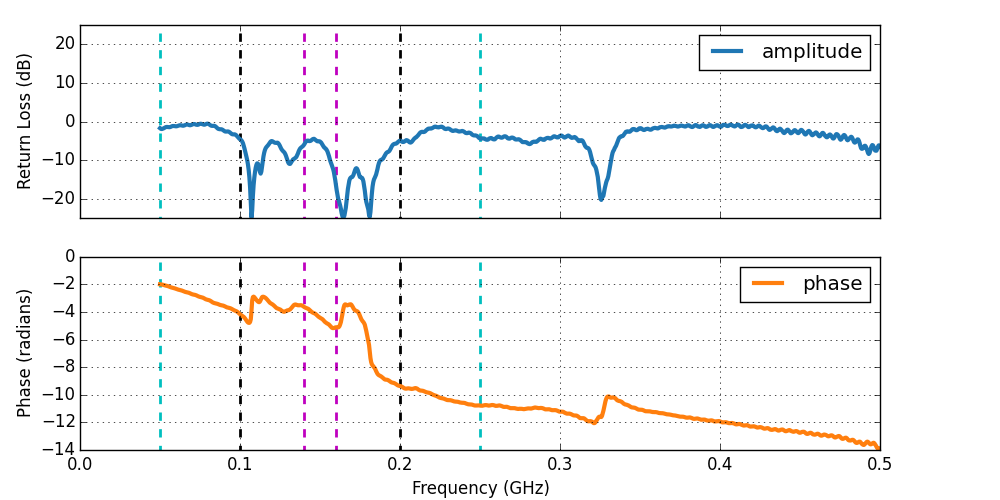
\includegraphics[totalheight=0.4\textheight]{plots/frequency_amp_phase_fullbw.png}
\caption{Amplitude and phase of the measured return loss. Colored dashed lines
mark three different frequency bands: $140-160MHz$ (typical power spectrum bandwidth), $100-200MHz$ (PAPER bandwidth), and
$50-250MHz$ (HERA bandwidth).}
\label{fig:freq}
\end{figure}

Frequency domain data, as shown in Figure \ref{fig:freq}, can be Fourier-transformed to compute the return loss in the delay domain. Because the measured data is band-limited between $50$ to $500MHz$, it is analogous to multiply the measured data by a square window function. Then in delay domain, the response would be convolved with a $sinc$ function. This may result in excess power at high
delays due to the sidelobes of the $sinc$ function. Hence, appropriate windowing of the measured data set is necessary before taking the Fourier transform.
We have chosen a Hamming window for our analysis, and its effectiveness of this
window function compared to others is illustrated in Figure
\ref{fig:window}. 

As mentioned in Section \ref{sec:theory}, there is a mismatch in amplitude
between the reflections that we measure (originating from the FieldFox pulse)
and reflections produced by sky signal. The reflections that we measure (at high
delays) must be lowered by a factor to represent weaker reflections that would
occur after most of the sky signal is received by the feed. For our
compensation, we multiply our entire delay spectrum by its DC component, which is the feed reflection coefficient $\Gamma_{f}$, and also divide by ($1-\Gamma_{f}$). In other words, these correction factors equate Equation \ref{eqn:ratio2} with Equation \ref{eqn:ratio1}. 
We note that this correction is only accurate at high delays where our
reflections of interest occur. At low delays, our spectrum amplitude should be
increased to represent the original sky signal, but we do not apply this
correction because it is not relevant to our analysis.

\begin{figure}[H]
\centering
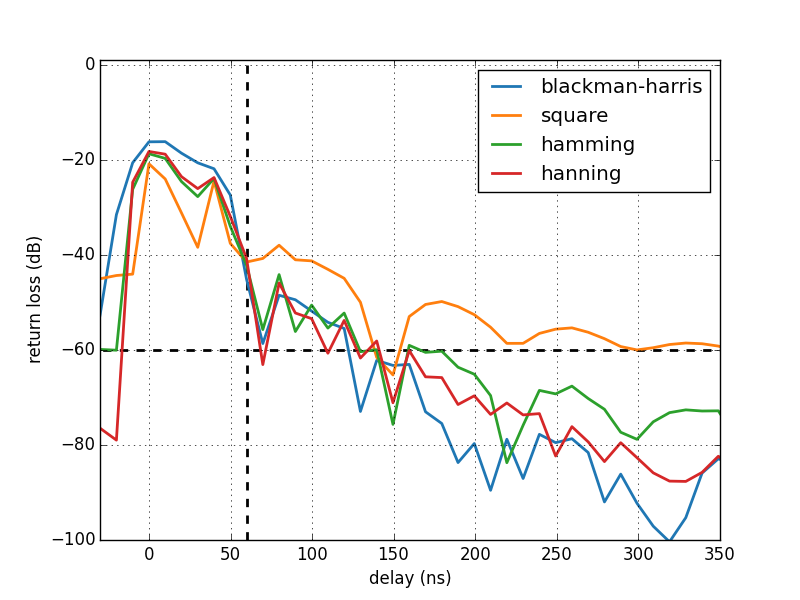
\includegraphics[totalheight=0.41\textheight]{plots/bh_vs_sq.png}
\caption{Delay plot produced for the PAPER bandwidth ($100MHz-200MHz$) by taking the Fourier transform of the measured return loss using four different window functions: Blackman-Harris, square, Hamming, and Hanning.}
\label{fig:window}
\end{figure}

\section{Results}

Figure \ref{fig:freq} shows the return loss for a frequency bandwidth of $50$ to
$500MHz$. This measurement was taken with the feed suspended at $4.26m$, which
was our closest measurement to the actual focal height.  Because the return
loss is the ratio of the power received to the power transmitted, higher
reflections can clearly be seen outside of the PAPER bandwidth. This is not
surprising, since the feed is tuned specifically for PAPER. The return loss
minima are locations where our feed is well-matched to free space.

In Figure \ref{fig:3bands}, the return loss we measure is plotted versus delay
for three chosen bandwidths: the HERA bandwidth, the PAPER bandwidth, and a
typical power spectra bandwidth when using a Hamming window function. Two
additional measurements, using data taken in 2014 with the first prototype HERA
dish near Berkeley, CA, are also plotted using two different bandwidths. One of
the main differences between the Green Bank and Berkeley measurements is that
the feed was not encompassed in a cage for the Berkeley data (only a backplane). Additionally, the $50-1000MHz$ data taken in Berkeley was
Fourier-transformed internally by the measuring device, while the $100-200MHz$
data is analyzed post-measurement in the same way as the Green Bank data. 

\begin{figure}[ht!]
\centering
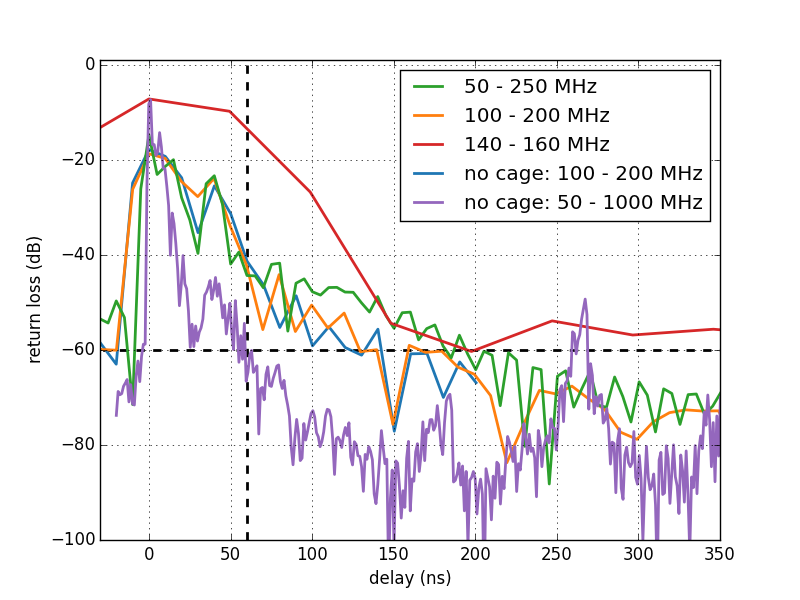
\includegraphics[totalheight=0.41\textheight]{plots/delay3_window.png}
\caption{Delay plots produced using a Hamming window function for 5 different cases. Three of the cases correspond to measurements taken in Green Bank for three frequency bandwidths: $50MHz-250MHz$ (HERA bandwidth), $100MHz-200MHz$ (PAPER bandwidth), and $140MHz-160MHz$ (typical power spectrum bandwidth). Two of the cases correspond to measurements taken in 2014 of the first prototype HERA dish in Berkeley (without a feed cage). Of these, we plot data for two frequency bandwidths: $100MHz-200MHz$ (PAPER bandwidth), and $50MHz-1000MHz$ (full bandwidth used by the VNA). For the PAPER bandwidth data, we follow the same Fourier-transform analysis as the others, while the full bandwidth data is produced directly by the VNA. The black dashed lines illustrate our ``60 by 60" specification.}
\label{fig:3bands}
\end{figure} 

From the plot, we see that the delay response of a feed is dependent on the band chosen for the Fourier transform.  As one might expect, in regions
where the feed return loss is low, reflections are minimized.  Thus, we cannot ignore that these measurements were performed
using a PAPER-style feed tuned for efficient operation over a $100-200MHz$ bandwidth.  Fourier transforms taken over wider bands
become dominated by the feed performance in regions outside the operating band, making the resultant delay profiles less relevant
for the power spectrum performance of the HERA instrument.  Conversely, when performing Fourier transforms over much 
narrow bands (the windowed $20MHz$ bands typical of PAPER analysis), the width of the resulting delay profile
becomes dominated by sidelobes of low delay emission interacting with the narrow bandwidth kernel.  
Although this may appear to be a relevant performance metric
for PAPER-style power spectrum analysis, such an analysis typically pre-filters out low-delay emission using wide bandwidths precisely to avoid
sidelobes from low-delay emission.  Hence, the most relevant delay-spectrum performance profile is that taken using the $100-200MHz$ band.

In the $100-200MHz$ delay profile, we see a delay response of $-50dB$ at $60ns$, which slopes down to $-60dB$ at $\sim120ns$.  Because
this does not achieve $-60dB$ attenuation at $60ns$, this indicates that the HERA system under test does not meet specification. However, we can learn additional information by evaluating
different feed components. 

\begin{figure}[ht!]
\centering
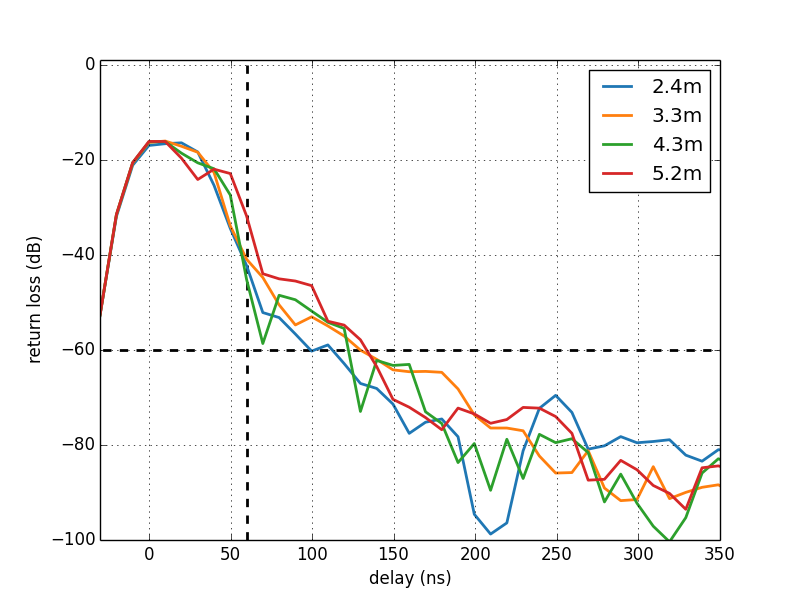
\includegraphics[totalheight=0.41\textheight]{plots/delay_heights_paper.png}
\caption{Delay plots produced using a Hamming window function for 4 different feed heights and the PAPER bandwidth ($100MHz-200MHz$). The black dashed lines illustrate our ``60 by 60" specification.}
\label{fig:elevator}
\end{figure}

Figure \ref{fig:elevator} is again a delay plot of the return loss, but for
four different feed suspension heights. We use the PAPER bandwidth and note
that the measurements are near identical at low delays, implying that low delay
reflections are caused primarily by reflections within the feed cage. However,
at higher delays we notice discrepancies between the different heights.

In addition, Figure \ref{fig:outofthedish} presents measurements taken of the feed
away from the dish. Echosorb is placed under the feed for some of the
measurements, with the expectation that it will prevent any reflections off the
ground. Measurements are also taken of the feed inside its metal cage in
various configurations. It is shown that the feed performs best without the cage and with the absorber. 


From these various measurements, we find that the feed itself is responsible for a significant portion of the structure up to $60ns$ and
that the cylindrical cage may be contributing up to $20ns$ to the width of the delay profile. We note that this depends strongly
on its coupling to structures around it. Structure beyond $60ns$ appears to scale
with the height of the feed above the dish, making reflections off the dish the likely culprit.

\begin{figure}[H]
\centering
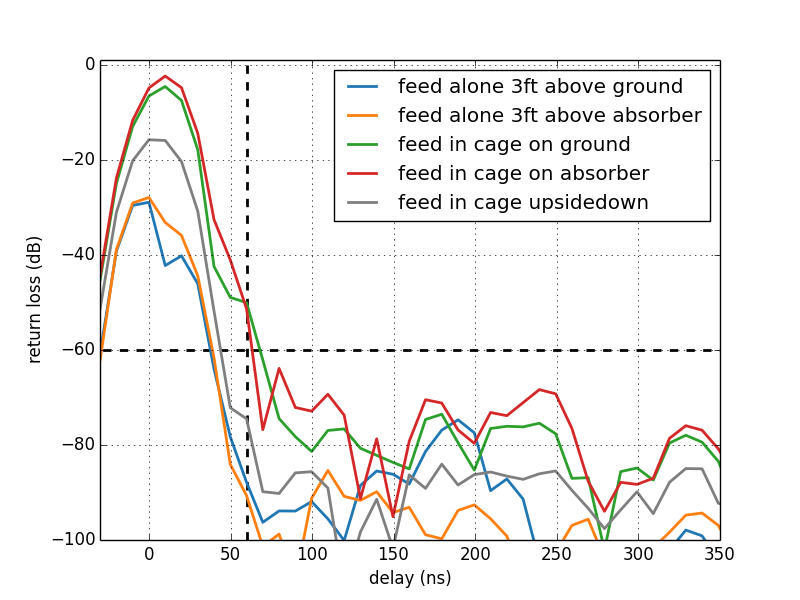
\includegraphics[totalheight=0.41\textheight]{plots/delay_feed.png}
\caption{Delay plots produced using a Hamming window function for different lone feed configurations and the PAPER bandwidth ($100MHz-200MHz$). The black dashed lines illustrate our ``60 by 60" specification.}
\label{fig:outofthedish}
\end{figure}

\section{Conclusion}

The delay-domain performance of the HERA dish is central to HERA's function as a power spectrum instrument.
As we have seen, reflectometry measurements can help characterize HERA's performance in this domain, and
as Equation \ref{eqn:ratio1} shows, these measurements must be adjusted for a difference in transmission/reflection
at the first feed encounter in order to be interpreted as the delay response of a feed relative to an incident
plane wave from the sky.  We also see that the choice of windowing function is critical for accurately measuring the
antenna delay response at higher delays, where sidelobes from much higher amplitude responses at small delays can easily
dominate.  We find Hamming, Hanning, and Blackman-Harris windows to be generally adequate while square windowing functions are not.
Given the critical nature of the windowing function, we recommend that all reflectometry measurements be performed in the
frequency domain, so that the data analyst can manually implement the Fourier transform with the appropriate window.

Taken all together, we summarize that the first version of the HERA dish, with a PAPER-style feed and cylindrical cage, is close to meeting
specification, but will require additional work to fall below $-60dB$ at $60ns$.  Given that the width of the delay response is a convolution
of the feed response and the dish reflections, it is not possible to perfectly decouple the response of the feed from that of the dish.
It may be possible to achieve enough of a reduction to meet specification by modifying the feed.
Given that previous measurements using a PAPER feed with a simple backplane exhibit structure above $-60dB$ at $60ns$,
we deduce that these advances will most likely require improving the feed return loss.  We also recommend re-investigating the scattering
cone for reducing standing waves between the feed and dish.  Finally, given the proximity of our measurements to the rough 
specification that was adopted for 
HERA of $-60dB$ attenuation at $60ns$, we recommend reinvestigating this specification to determine more accurately the impact of 
the element's current delay performance on HERA science.  We suspect that, at the level of $-50dB$ at $60ns$ and $-60dB$ at $120ns$, this
performance may indeed be adequate for the delay-domain power spectrum analysis for which HERA has been optimized.

\bibliographystyle{apj}
\bibliography{biblio.bib}
%\begin{thebibliography}{}
%
%\bibitem[Parsons \& Backer(2009)]{ParsonsBacker2009}
%Parsons, A., \& Backer, D. 2009, \apj, 138, 219
%\bibitem[Parsons et al.(2012)]{Parsons2012}
%Parsons, A., \& Pober, Jonathan C., \& Aguirre, James E., \& Carilli, Christopher L., \& Jacobs, Daniel C., \& Moore, David F. 2012, \apj 756, 165
%\end{thebibliography}{}

\end{document}


%\begin{eqnarray}
%V e^{i\phi}(\nu) & = & \int |A_{f}|^{2}|V_{sky}|^{2}|exp({2\pi i \nu \vec{b}.\hat{s} \over c} ) d\Omega \nonumber\\
%&& +  \int |A_{f}|^{2}|V_{sky}|^{2} |(1-\Gamma_{f})|^{2}|\Gamma_{f}|^{2}|\Gamma_{d}|^{2} exp({2\pi i \nu \vec{b}.\hat{s} \over c} ) d\Omega \nonumber\\
%&& + \int |A_{f}|^{2}|V_{sky}|^{2}| 2 \Re \left ((1-\Gamma_{f})\Gamma_{f}\Gamma_{d} e^{i\Phi} \right)exp({2\pi i \nu \vec{b}.\hat{s} \over c} ) d\Omega
%\label{eq8}		        
%\end{eqnarray}

 
%\subsection{Effect of first reflection on the delay spectrum}
%We define $B(\vec \theta, \nu) =  A^{2}(\vec \theta, \nu) $ as the cross power pattern of the interferometer and $\Sigma_{rr}(\nu), \Sigma_{dr}(\nu)$ are the correlation coefficient between the two reflected signals in each antenna and the direct signal of one antenna with the reflected signal from the other antenna in the uv plane i.e, 

%\begin{equation}
%\Sigma_{rr}(\nu) =  \left [ |(1-\Gamma_{f})|^{2}|\Gamma_{f}|^{2}|\Gamma_{d}|^{2} \right ]
%\end{equation}

%\begin{equation}
%\Sigma_{dr}(\nu) = \left [ 2 \Re \left ((1-\Gamma_{f})\Gamma_{f}\Gamma_{d} e^{i\Phi} \right) \right]
%\end{equation}

%and $\Delta \tau$ is the additional delay each reflected component suffers in addition to the intrinsic geometric delay 
%$\tau_{g}$. Therefore, $\Sigma(\vec \theta, \nu) = B(\vec \theta, \nu) \left [ 1+\Sigma_{rr} +\Sigma_{dr} \right]$

%As given in equation \ref{eq3}, the Fourier transform of this visibility spectrum along the frequency axis results in the delay spectrum. Hence, the all sky integrated delay spectrum could be written as, 
%\begin{eqnarray}
%\mathcal{F} \left [V e^{i\phi}\right] & = & \int \left [\int B I_{sky}exp({2\pi i \nu \vec{b}.\hat{s} \over c} ) d\Omega \right ] exp\left[ -2 \pi i\nu \tau \right] d\nu \nonumber\\
%&& + \int \left [  \int B I_{sky} \Sigma_{rr} exp({2\pi i \nu \vec{b}.\hat{s} \over c} ) d\Omega \right] exp\left[ -2 \pi i\nu \tau \right] d\nu  \nonumber\\
%&& +\int \left [ \int B I_{sky} \Sigma_{dr} exp({2\pi i \nu \vec{b}.\hat{s} \over c} ) d\Omega \right ] exp\left[ -2 \pi i\nu \tau \right] d\nu \nonumber\\	
%&& + \int \left [  \int |A_{f}|^{2}|V_{sky}|^{2} |(1-\Gamma_{f})|^{2}|\Gamma_{f}|^{2}|\Gamma_{d}|^{2} exp({2\pi i \nu \vec{b}.\hat{s} \over c} ) d\Omega \right] exp\left[ -2 \pi i\nu \tau \right] d\nu  \nonumber\\
%&& +\int \left [ \int |A_{f}|^{2}|V_{sky}|^{2} 2 \Re \left ((1-\Gamma_{f})\Gamma_{f}\Gamma_{d} e^{i\Phi} \right)exp({2\pi i \nu \vec{b}.\hat{s} \over c} ) d\Omega \right ] exp\left[ -2 \pi i\nu \tau \right] d\nu \nonumber\\			
%			& = & \int \left [\int B I_{sky} exp({2\pi i \nu \tau_{g}} ) dl dm \right ] exp\left[ -2 \pi i\nu \tau \right] d\nu \nonumber\\
%&& + \int \left [  \int B I_{sky} \Sigma_{rr} exp({2\pi i \nu \tau_{g}} ) dl dm \right] exp\left[ -2 \pi i\nu \tau \right] d\nu  \nonumber\\
%&& +\int \left [ \int B I_{sky} \Sigma_{dr} exp({2\pi i \nu \tau_{g}} ) dl dm \right ] exp\left[ -2 \pi i\nu \tau \right] d\nu \nonumber\\
%\label{eq9}
%\end{eqnarray}
%
%\begin{eqnarray}			
%\mathcal{F} \left [V e^{i\phi}\right] & = & \left [ B(\tau)\ast I_{sky}(\tau) \right ]\ast \delta(\tau+\tau_{g}) \nonumber\\
%		&& +  \left [ B(\tau)\ast I_{sky}(\tau)* \Sigma_{rr}( \tau) \right ]\ast \delta(\tau+\tau_{g}) \nonumber\\
%		&& +  \left [B(\tau)\ast I_{sky}(\tau)* \Sigma_{dr}( \tau) \right ]\ast \delta(\tau+\tau_{g}+ \Delta \tau)\nonumber\\
%\label{eq10}
%\end{eqnarray}

 %In words, the Fourier transform of the visibility contributed by any two voltage components from two antennas with no mutual delay is centred at a delay $\tau = \tau_{g}$ in the delay spectrum whereas any two voltage components from two antennas components having a mutual delay of $\Delta \tau$ will be centred at $\tau_{g} +\Delta \tau$. The correlation between the reflected signal  from the feed and subsequently from the dish with the direct signal thus extends the foreground response to delays beyond the maximum geometric delay for a given baseline and contaminates the delay mode where 21~cm delay spectrum could potentially be detected. Also, any reflections arriving at the feed at any non-zero  value of the delay $\Delta \tau$ which could be the result of reflections from the feed structures would generate non zero delay response at those delays. 

